%--------------------------------------------------
\section{Código fuente PHP}
\begin{itemize}
\item Sin excepción todo código de PHP debe de seguir los estándares PSR-1 y PSR-2 definidos por la comunidad de PHP. Destacando los puntos:

	\begin{itemize}
		\item PSR-1
			\begin{itemize}
				\item Los archivos deben usar solamente las etiquetas <?php.
				\item Los archivos deben usar solamente el formato de codificación UTF-8.

				\item Namespaces y clases deben seguir un "autoloading" PSR: [PSR-0, PSR-4].

				\item El nombre de las clases debe ser declarado en StudlyCaps.
				\item El nombre de los métodos debe ser declarado en camelCase.
			\end{itemize}
			
			\item PSR-2
			\begin{itemize}
				\item El código debe seguir la guía de estilo del PSR-1

				\item El código debe tener 4 espacios de indexación, no tabs.

				\item Las palabras clave de php deben de ir en minúsculas.

				\item Debe de haber un límite en el número de líneas por método, el total de líneas no debe pasar las 120 y se recomienda que cada línea tenga 80 caracteres o menos.

				\item Se debe dejar una línea en blanco después del namespace y del bloque de declaraciones de use.

				\item Las llaves de apertura de los métodos y clases deben de ir en la línea siguiente y la llave de cierre debe de ir en la línea siguiente después de la declaración del cuerpo.

				\item Las llaves de apertura de las estructuras de control deben de ir en la misma línea y la llave de cierre debe de ir en la línea siguiente después de la declaración del cuerpo.

				\item La etiqueta de cierre ?\textgreater del archivo (\textless ?php) debe ser omitida del contenido si el archivo sólo contiene código PHP. (Figura 2.1)
				
				\item 								
				\item Sin excepción todos los métodos y clases los debe contener una descripción. De acuerdo a la documentación no oficial que propone phpDocumentor.

				
				\item PHPDoc es un estándar informal para comentar coding en php. Existen diversas etiquetas disponibles. En la figura 2.2 se muestra la implementación.

			\end{itemize}
	\end{itemize}
\end{itemize}

				\begin{figure}[htbp!]
		\centering
			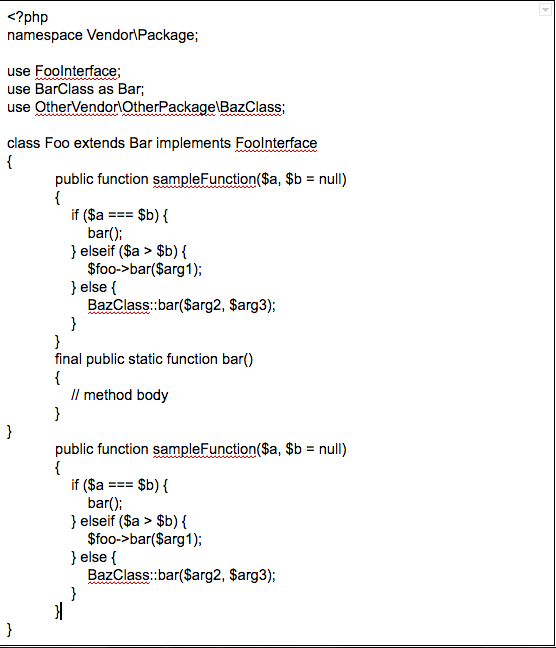
\includegraphics[width=1\textwidth]{images/ejemploCodigo1}
		\caption{Ejemplo de código 1}
	\end{figure}
				

				\begin{figure}[htbp!]
		\centering
			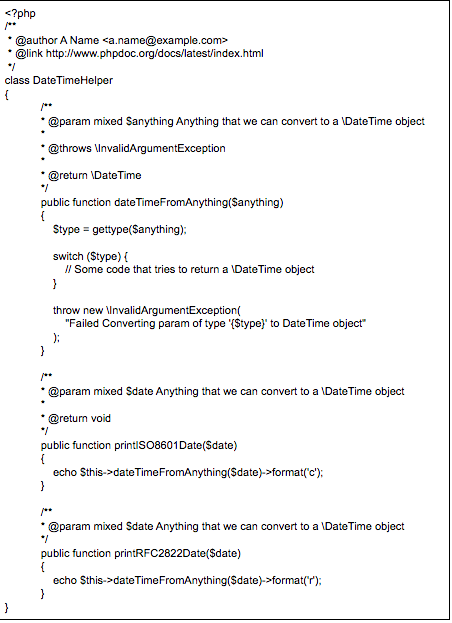
\includegraphics[width=1\textwidth]{images/ejemploCodigo2}
		\caption{Ejemplo de código 2}
	\end{figure}
				
\section{Código fuente de Symfony}
\subsection{Controles}
\begin{itemize}
\item Definidos en src/AppBundle/Controller

\item Se deben crear por actor dentro de una carpeta Actor/ y el nombre del archivo debe tener la terminación Controller

\end{itemize}
\subsection{Documentos}
\begin{itemize}
\item Definidos en src/AppBundle/Document

\item Se deben crear por actor dentro de una carpeta Actor/ 

\end{itemize}
\subsection{Repositorios}
\begin{itemize}
\item Definidos en src/AppBundle/Repository

\item Se deben crear por actor dentro de una carpeta Actor/ y el nombre del archivo debe tener la terminación Repository

\end{itemize}
\subsection{Formularios}
\begin{itemize}
\item Definidos en src/AppBundle/Form/Type/

\item Se deben crear por actor dentro de una carpeta Actor/ y el nombre del archivo debe tener la terminación Type

\end{itemize}

\section{Variables}
Sin excepción los nombres de las variables deben de seguir el estilo lowerCamelCase.

\section{Contoles}
Se recomienda seguir la regla 5-10-20. La cual dice que se deberían definir 5 variables o menos, contener 10 acciones o menos e incluir 20 líneas de código o menos en cada acción.

\section{Métodos y funciones}
A no ser que se especifique lo contrario, los nombre de los métodos/funciones deben de colocarse en idioma inglés. Esto debido a que las palabras en inglés suelen requerir menos caracteres que las palabras en español (note la cantidad de letras usadas en estas variables obtenerUsuarios vs getUsers).
\newpage
\section{AngularJS}
La estructura de las carpetas para almacenar el código angular por módulo debe de ser la siguiente:
				\begin{figure}[htbp!]
		\centering
			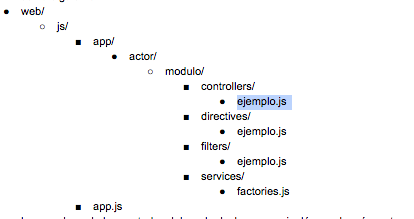
\includegraphics[width=1\textwidth]{images/estructura}
		\caption{Estructura AngularJS}
	\end{figure}

\begin{itemize}
	\item Los nombres de los controles deben de declararse en inglés, ser lo más corto posible, usar UperCamelCase y llevar el sufijo Ctrl, ejemplo UserCtrl, AdminCtrl.

	\item Por la estructura de la carpeta, no es necesario que los nombres de los archivos tengan terminaciones Controller, Filter, Directive o Factory.

	\item El nombre de los factories debe de declararse en inglés, ser lo más corto posible y usar UperCamelCase.

	\item Bajo ninguna circunstancia se usarán selectores de jQuery dentro de controles o providers.

	\item Si se requieren utilizar funciones de jQuery se deberá crear un directiva.

	\item Los nombres de las directivas deben de declararse en inglés, ser lo más corto posible y usar lowerCamelCase.

	\item Cada control, directiva, servicio y filtro, así como las funciones se deben de comentar, indicando el uso de la función y los parámetros que necesita, en caso de ser necesarios.

\end{itemize}

\section{JavaScript}

\begin{itemize}
\item Toda variable debe de ser declarada y de ser necesario inicializada, seguir la convención para javascript var myVar; y var myVar=1;

\item Los nombres de las variables deben de declararse en inglés, ser lo más corto posible, ser lo más descriptivas posibles y usar lowerCamelCase.

\item Todo el código javascript debe estar separado en un archivo dentro de la carpeta web/js

\end{itemize}

\section{CSS}
\begin{itemize}
	\item Se deben seguir los lineamientos de diseño de bootstrap

	\item Todo código css debe estar separado en un archivo dentro de la carpeta web/css.

\end{itemize}
% - - - - - - - - - - - - - - - - - - - - - - - - -
